\documentclass[11pt]{article} 



\makeatletter
\renewcommand\section{\@startsection{section}{1}{\z@}%
                                  {-3.5ex \@plus -1ex \@minus -.2ex}%
                                  {2.3ex \@plus.2ex}%
                                  {\normalfont\large\bfseries}}
\makeatother

\addtolength{\oddsidemargin}{-.875in}
\addtolength{\evensidemargin}{-.875in}
\addtolength{\textwidth}{1.75in}
\addtolength{\topmargin}{-.875in}
\addtolength{\textheight}{1.75in}


\usepackage{amssymb}
\usepackage{amsmath}
\usepackage{amsthm}
\usepackage{graphicx,caption,subcaption}


\usepackage{titling}
\setlength{\droptitle}{-6em}
\posttitle{\par\end{center}\vspace{-4.8em}}

\newcommand{\R}{{\ensuremath{\mathbb{R}}} }
\newcommand{\Q}{{\ensuremath{\mathbb{Q}}} }
\newcommand{\C}{{\ensuremath{\mathbb{C}}} }
\newcommand{\N}{{\ensuremath{\mathbb{N}}} }
\newcommand{\Z}{{\ensuremath{\mathbb{Z}}} }

\newcommand{\sexion}{\addtocounter{section}{1} }


\newcommand{\hint}[1]{{(\emph{Hint:} #1)}} %This line shows hints
%\newcommand{\hint}[1]{} %Use this line to hide all hints


\usepackage{fancyhdr}
\pagestyle{fancyplain}
\renewcommand{\headrulewidth}{0pt}

\begin{document}

%\lhead{}
\rhead{2-D Mixing}
\section{Problem}
We have two bucket each full, and containing 500 gal water. Pure water enters the first bucket at a rate of 5 gal / sec, mixes perfectly, and flows into the second bucket at a rate of 5 gal / sec. Mixed water leaves the second bucket at a rate of 5 gal / sec. Initially the first bucket has 100 lbs salt and the second has pure water.

\section{General Solution}

As usual for a mixing problem we want to write 
\[ \mbox{Rate} = \mbox{Rate In} - \mbox{Rate Out}\]
For the first bucket this is just 
\[x'_0(t) = 0 - 5 \frac{gal}{sec} \cdot \frac{x_0(t) lbs}{500 gal}\]
The second is
\[x'_1(t) =  5 \frac{gal}{sec} \cdot \frac{x_0(t) lbs}{500 gal} -  5 \frac{gal}{sec} \cdot \frac{x_1(t) lbs}{500 gal}\]

So we have the matrix system
\[\left( \begin{array}{cc} - \frac{1}{100} & 0 \\ \frac{1}{100} & - \frac{1}{100} \end{array} \right) \left( \begin{array}{c} x_0 \\ x_1 \end{array} \right) = \left(\begin{array}{c}x_0' \\ x_1' \end{array} \right) \]

Now that we have a system we need to compute the eigenvalues. Write the Characteristic equation
\[ | A - \lambda I  | = \left| \begin{array}{cc} - \frac{1}{100} - \lambda& 0 \\ \frac{1}{100} & - \frac{1}{100} - \lambda \end{array} \right|  =  \left( - \frac{1}{100} - \lambda \right) ^2 = 0\]
So, we have one real eigenvalue $\lambda = -1/100$ with multiplicity 2. Now to find a corresponding eigenvector we just compute
\[ \left( \begin{array}{cc} - \frac{1}{100} & 0 \\ \frac{1}{100} & - \frac{1}{100} \end{array} \right)  \left( \begin{array}{c} v_0 \\ v_1 \end{array} \right)  = -\frac{1}{100} \left( \begin{array}{c} v_0 \\  v_1 \end{array} \right)\]
So, $v_0 = 0$. Let's choose our eigenvector to be
\[v = \left( \begin{array}{c} 0 \\ 1 \end{array} \right)\]
Now we want to find a `generalized eigenvector' $w$ satisfying
\[(A - \lambda I ) w = v\]
Computing, we must have
\[   \left( \begin{array}{cc} - \frac{1}{100} - (- \frac{1}{100}))& 0 \\ \frac{1}{100} & - \frac{1}{100} - (- \frac{1}{100}) \end{array} \right)  \left( \begin{array}{c} w_0 \\ w_1 \end{array} \right) =  \left( \begin{array}{c} 0 \\ 1 \end{array} \right)\]
or equivalently,
\[\frac{1}{100} w_0 = 1\]
So let's choose 
\[w = \left( \begin{array}{c}100\\ 0 \end{array} \right)\]
Now we can write the general solution using our formula as
\[x(t) = e^{\lambda t} \left( ( C_1 + C_2 t) v   + C_2  w \right) = e^{-  t / 100} \left( ( C_1 + C_2 t)  \left( \begin{array}{c}0\\ 1 \end{array} \right)  + C_2  \left( \begin{array}{c}100\\ 0 \end{array} \right) \right)  \]

\section{Particular Solution / Analysis}
We can split the general solution back into two equations:
\[ x_0(t) = 100 C_2  e^{-t / 100}  \quad x_1(t) = (C_1 + C_2 t) e^{-t /100}\]
Recall that we had as initial condition $x_0(0) = 100, x_1(0) = 0$. The first gives us
\[x_0(0) = 100 C_2  e^{0  / 100} = 100 \Rightarrow    C_2 = 1\]
and from the second we have
\[ x_1(0) = (C_1 + C_2  \cdot 0) e^{0 /100} =   C_1 = 0   \]
So the particular solution is:
\[ x_0(t) = 100  e^{-t / 100}\]
\[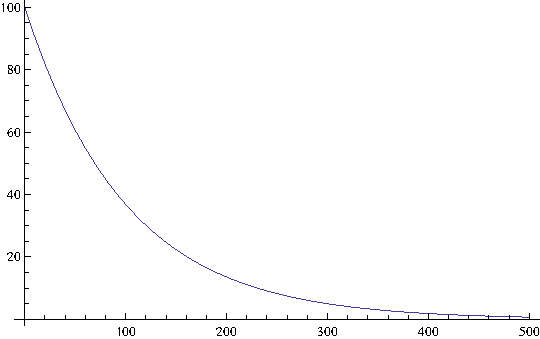
\includegraphics{plot1}\]
\[ x_1(t) =  t e^{-t /100} \]
\[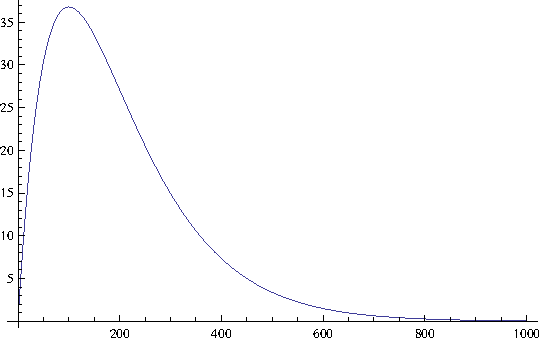
\includegraphics{plot2}\]
\end{document}
